\setchapterimage{west_div_roux_cropped}
\setchapterpreamble[u]{\margintoc}
\chapter{Divertor inventory estimation}\label{Chapter4}\labch{Chapter4}
\labch{Divertor inventory estimation}

% \section{Introduction}

This Chapter focusses on the estimation of the H inventory in the divertors of WEST and ITER.
This estimation relies on monoblocks behaviour law computed in \refch{Chapter3}.
This behaviour law allows rapid evaluations of the monoblocks H inventory.
Inputs are taken from SolEdge3X-EIRENE \cite{bufferand_three-dimensional_2019} and SOLPS-ITER \cite{kaveeva_solps-iter_2020} plasma simulations.
The influence of several control parameters is investigated: the input power (\textit{ie} how much heating power is injected in the plasma), the gas puffing rate (used in most tokamaks to increase the plasma density \cite{zweben_effect_2014}), and the divertor pressure of neutral particles in ITER.


\section{Methodology}
\begin{figure}[h!]
    \centering
    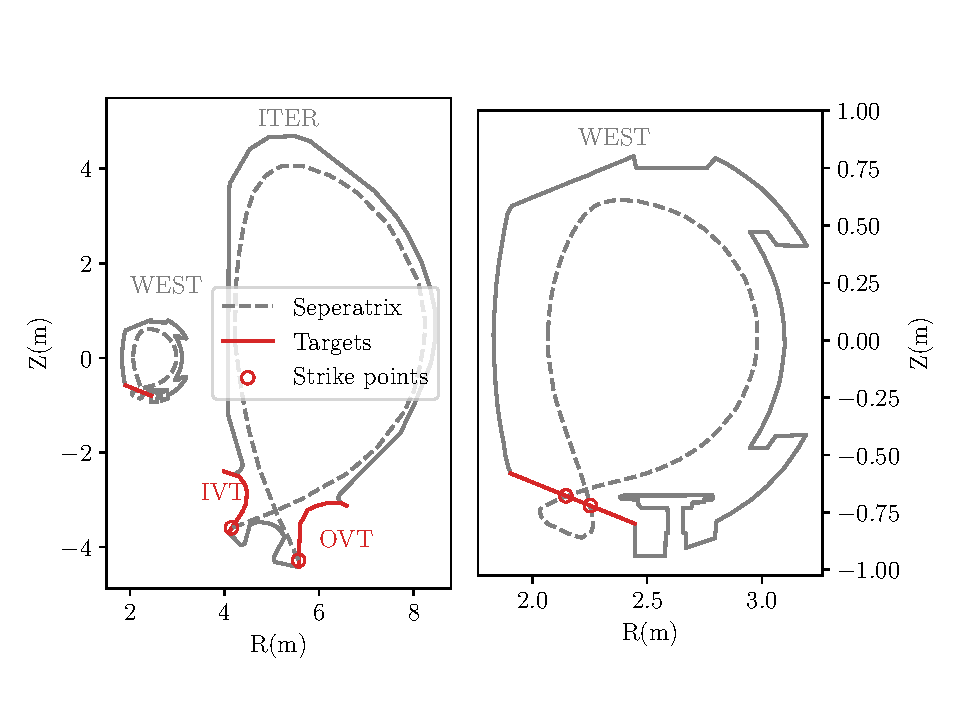
\includegraphics[width=0.95\linewidth]{Figures/divertor/coordinates.pdf}
    \caption{Geometry of WEST and ITER divertors}
    \label{fig: reactors}
\end{figure}

% The H inventory of the WEST and ITER divertors will be computed by making use of a database of FESTIM simulations of H transport in ITER-like monoblocks from which a behaviour law is extracted using a gaussian regression process from the inference-tools python package \sidecite{chris_bowman_c-bowmaninference-tools_2020}.
% These simulations model H transport in monoblocks for a fixed plasma exposure duration of \SI{e7}{s}.
% This corresponds to approximately 25 000 concatenated ITER discharges of \SI{400}{s} each.
% As shown in \sidecite{hodille_modelling_2021}, this approximation does not affect the H inventory in monoblocks with the current conditions.

% These results are then interfaced with the exposure conditions obtained with the plasma simulations performed with the codes SOLPS \sidecite{kaveeva_solps-iter_2020} and SOLEDGE \sidecite{bufferand_three-dimensional_2019}.


\subsection{Plasma simulations}
This Section describes the parameters of the plasma simulations.
For the SolEdge3X-EIRENE runs, the puffing rate and the input power were used as control parameters.
For SOLPS-ITER calculation, the divertor neutral pressure is the control parameter.
\subsubsection{SolEdge3X-EIRENE runs}
The Lower-Single-Null magnetic configuration used for the 2D simulations in SolEdge3X-EIRENE transport code (v588.165) are based on the experimental WEST plasma discharge \#54903 at $T_\mathrm{flat-top} = \SI{8}{s}$ (see Figure \ref{fig: reactors}).
In order to get as many divertor conditions as possible, the puffing rate was varied from \SI{4.5e20}{molecule.s^{-1}} to \SI{4.72e21}{molecule.s^{-1}} and the input power from \SI{0.449}{MW} to \SI{2.5}{MW}.
The setup parameters of the simulation are listed in Table \ref{tab: my_tab}.
$R_\mathrm{wall}$ is the recycling coefficient of main chamber wall, $R_\mathrm{pump}$ is the recycling coefficient of the pump, $D_\mathrm{m}$ is the cross-field mass diffusivity perpendicular to the flux surface, $\nu$ is the momentum diffusivity, $\chi_e$ and $\chi_i$ are the heat flux diffusivity for electrons and ions, respectively.
The gas puff position is set inside the private region and the pump position is set under the baffle.

\begin{table}[!ht]
    \centering
    \caption{Setup parameters used in the SOLEDGE3X simulations}
    \begin{tabular}{L{0.4\linewidth}  R{0.4\linewidth}}
    \hline \\
    Plasma composition & Deuterium, no impurity \\
    \\
    Recycling coefficients &  $R_\mathrm{wall} = 0.99$ \\
     & $R_\mathrm{pump} = 0.95$ \\
    \\
    SOL input power & from \SI{0.449}{MW} to \SI{2.5}{MW} \\
    \\
    Gas puffing rate & from \SI{4.5e20}{molecule.s^{-1}} to \SI{4.72e21}{molecule.s^{-1}} \\
    \\
    Drifts & - \\
    \\
    Transport coefficients & $D_\mathrm{m} = \SI{0.3}{m^2.s^{-1}}$ \\
     & $\nu = \SI{0.3}{m^2.s^{-1}}$ \\
     & $\chi_e = \chi_i = \SI{1.0}{m^2.s^{-1}}$ \\
    \end{tabular}
    \label{tab: my_tab}
\end{table}


\subsubsection{SOLPS runs}
Several ITER cases were taken with divertor neutral pressures varying from \SI{1.8}{Pa} to \SI{11.2}{Pa}.
These SOLPS \sidecite{kaveeva_solps-iter_2020} scenarios can be found in the ITER Integrated Modelling Analysis Suite (IMAS) database \sidecite{imbeaux_design_2015, park_assessment_2020}.
The nine simulations used in this work are labelled 122396, 122397, 122398, 122399, 122400, 122401, 122402, 122403 and 122404.
These have been run in baseline burning plasma conditions (Q=10) and with an averaged separatrix Ne concentration of around \SI{0.6}{\%} \sidecite{pitts_physics_2019}.


\begin{figure}[h!]
    \centering
    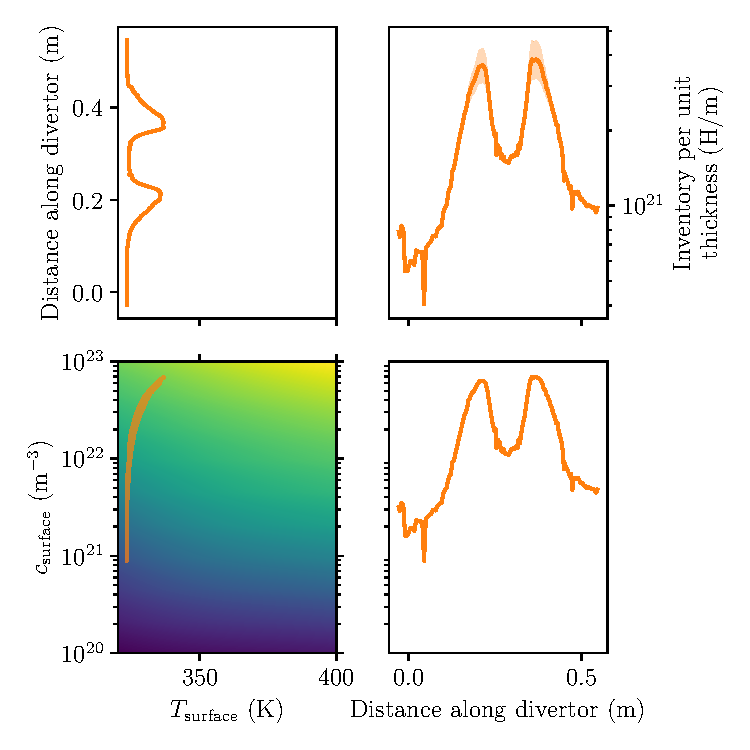
\includegraphics[width=\linewidth]{Figures/divertor/example.pdf}
    \caption{Method of divertor H inventory estimation based on the surface concentration, the surface temperature and the behaviour law obtained in \refch{Chapter3}.}
    \label{fig: behaviour law example}
\end{figure}

\subsection{Estimation of exposure conditions}

\begin{figure*}[h]
    \centering
    \begin{subfigure}{0.5\linewidth}
        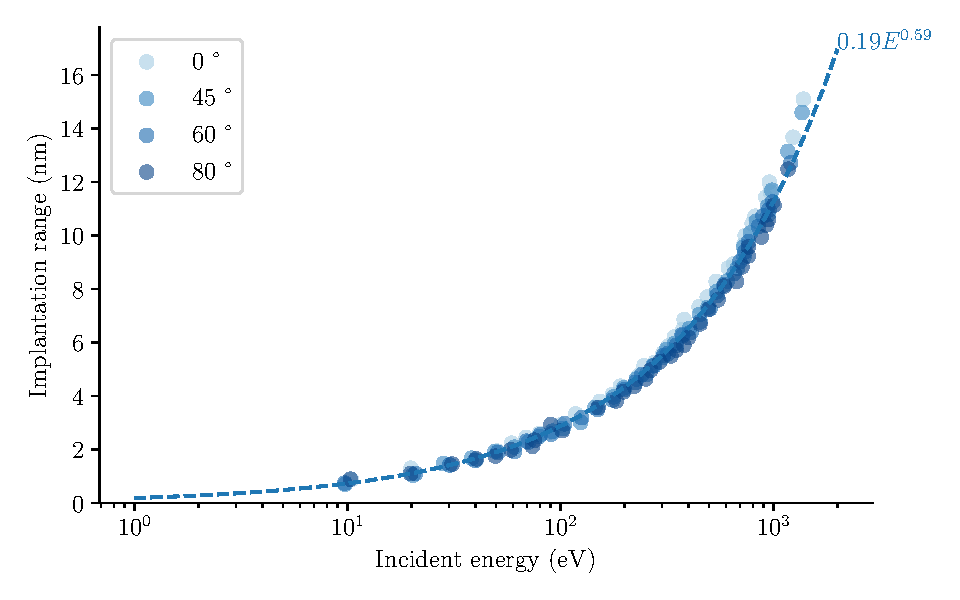
\includegraphics[width=\linewidth]{Figures/divertor/implantation_range.pdf}
        \caption{Implantation range $R_p$}
        \label{fig: implantation range vs energy}
    \end{subfigure}%
    \begin{subfigure}{0.5\linewidth}                          
        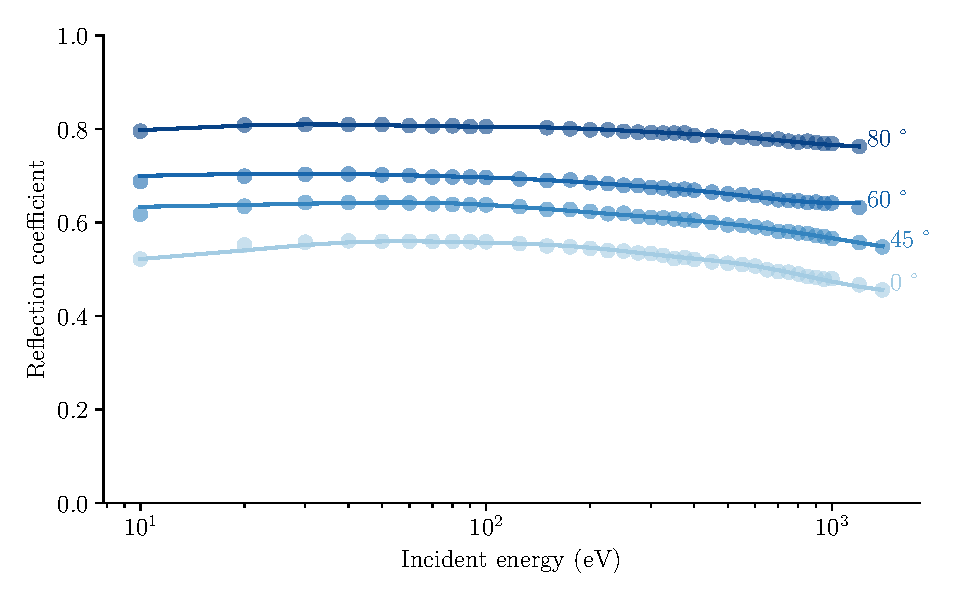
\includegraphics[width=\linewidth]{Figures/divertor/reflection_coeff.pdf}
        \caption{Reflection coefficient $r$}
        \label{fig: reflection coeff vs energy}
    \end{subfigure}
    \caption{Evolution of the implantation range and the reflection coefficient as a function of incident energy $E$ and angle of incidence.}
\end{figure*}

According to the behaviour law obtained in Chapter \ref{Chapter3}, the temporal evolution of the H inventory along the divertors can be estimated from the surface concentration of mobile hydrogen and surface temperature (see Figure \ref{fig: behaviour law example}).
% This inventory distribution can then be projected onto the whole divertor geometry for better visualisation (see Figure \ref{fig: top view}).

The distribution of the exposure conditions (angles of incidence, particles energies, particles fluxes and heat flux) are produced by SOLEDGE/SOLPS along the divertors of WEST and ITER (see Figures \ref{fig: reactors} and \ref{fig: behaviour law example}).
These exposure conditions are converted into distributions of surface temperature $T_\mathrm{surface}$ and surface hydrogen concentration $c_\mathrm{surface}$ by Equations \eqref{eq: thermal behaviour} and \eqref{eq: c_surface}.

\begin{equation}
    T_\mathrm{surface} = 1.1\times 10^{-4} \varphi_\mathrm{heat} + 323
    \label{eq: thermal behaviour}
\end{equation}
where $\varphi_\mathrm{heat}$ is the surface heat flux in \si{W.m^{-2}}.

The relation between the heat flux $\varphi_\mathrm{heat}$ and the surface temperature $T_\mathrm{surface}$ (see Equation \eqref{eq: thermal behaviour}) has been obtained from heat transfer simulations of ITER monoblocks (see Section \ref{monoblock thermal behaviour}).

\begin{equation}
    \label{eq: c_surface}
    c_\mathrm{surface} = \ (1 - r_\mathrm{atoms}) \ \frac{R_{p, \mathrm{atoms}} \ \varphi_\mathrm{atoms}}{D(T_\mathrm{surface})} + (1 - r_\mathrm{ions}) \nonumber \ \frac{R_{p, \mathrm{ions}} \ \varphi_\mathrm{ions}}{D(T_\mathrm{surface})}
\end{equation}

where the reflection coefficients $r_i$ and implantation depths $R_{p, i}$ in \si{m}, $\varphi_{i}$ are the particles fluxes in \si{m^{-2}.s^{-1}} and $D$ is the H diffusion coefficient in \si{m^{2}.s^{-1}}.

The implantation range $R_p$ and the reflection coefficient $r$ depend on the incident energy and angle of incidence of particles.
These relations can be obtained from SRIM \sidecite{ziegler_srim_2010} simulations (see Figure \ref{fig: implantation range vs energy}).
It was found that the angle of incidence had low influence on the implantation range.
$R_p$ can then be expressed (in \si{m}) as a function of the incident energy only (see Equation \eqref{eq: implantation range}).

\begin{equation}
    R_p = 1.9\times 10^{-10} E ^{0.59}
    \label{eq: implantation range}
\end{equation}
where $E$ is the incident energy in \si{eV}.

The evolution of the reflection coefficient $r$ can also be estimated with SRIM.
The reflection coefficient varies from around 0.5 at \SI{0}{^\circ} to 0.8 at \SI{80}{^\circ} (see Figure \ref{fig: reflection coeff vs energy}).
According to \sidecite{park_assessment_2020}, the incident angles for ions and atoms were assumed to be \SI{60}{^\circ} and \SI{45}{^\circ}, respectively.
It should be noted that since SRIM is based on the binary collision approximation, values around \SI{10}{eV} might not be fully valid.

All of these steps have been automated and packaged into a tool called divHretention.
divHretention can directly link SOLPS/SOLEDGE output files and produce a distribution of monoblock inventory as in Figure \ref{fig: behaviour law example}.
The source-code of the tool is under version control and openly available via Github under a MIT licence \cite{delaporte-mathurin_irfmdivhretention_2021}.
The divHretention python package is distributed via PyPi \cite{delaporte-mathurin_divhretention_nodate}.
Moreover, all the results obtained in this Chapter can be reproduced with the scripts available at \href{https://github.com/RemDelaporteMathurin/divHretention-Nucl.Fusion-2021}{https://github.com/RemDelaporteMathurin/divHretention-Nucl.Fusion-2021}.

\section{ITER results}

% \subsection{Influence of incident particle flux and ion energy on hydrogen inventory} \label{particle and energy}
% Incident particle flux $\varphi_\mathrm{inc}$ and ion energy $E$ have an impact on the amount of mobile particles implanted in the material but also on the heat load and therefore on the surface temperature of the monoblock.

% Assuming a source term with a narrow Gaussian distribution and a non-instantaneous recombination (characterised by a recombination coefficient $K$), the concentration $c_\mathrm{max}$ at the near surface is approximated by:

% \begin{equation}
%     c_\mathrm{max} =  \frac{\varphi_\mathrm{imp} \cdot R_p}{D(T_\mathrm{surface})} + \sqrt{\frac{\varphi_\mathrm{imp}}{K(T_\mathrm{surface})}}
%     \label{eq:cmax}
% \end{equation}

% where $\varphi_\mathrm{imp} = (1-r) \cdot \varphi_\mathrm{inc}$ is the implanted particle flux, $r$ is the particle reflection coefficient, $K$ is the recombination coefficient, and $R_p$ is the mean implantation depth in \si{m}.
% Details can be found in appendix \textcolor{black}{as Supplementary Material}.
% Many different values of the recombination coefficient $K$ for tungsten can be found in literature.
% For instance the widely used Anderl coefficient describes an endothermic recombination \sidecite{anderl_hydrogen_1990} whereas Ogorodnikova showed an exothermic recombination coefficient could be used to reproduce a set of experiments \sidecite{ogorodnikova_recombination_2019}.

% Facing the difficulty of an accurate choice for $K$ and following the recommendation of Causey \textit{et al} \sidecite{causey_hydrogen_2002}, an instantaneous recombination will therefore be assumed (\textit{ie} $K \rightarrow +\infty$).
% It is also worth noting that experiments by Bisson \textit{et al} \sidecite{bisson_dynamic_2015} support the fact that recombination is not the rate limiting step during the hydrogen release from polycrystalline tungsten after ion implantation.

% In the following, the concentration on $\Gamma_\mathrm{top}$ was set to $c_\mathrm{surface} = c_{\mathrm{max}}$ for the kinetics involved are really fast (see appendix of \sidecite{hodille_hydrogen_2018}) and $R_p$ is small compared to the monoblock dimensions.

% The heat load was assumed to evolve as a function of the incident particle flux $\varphi_\mathrm{inc}$ and $E$ as follow:

% \begin{equation}
%     \varphi_H = 2.2\cdot \varphi_\mathrm{inc} \cdot e \cdot (E + \SI{13.6}{eV})
%     \label{eq:phi_H}
% \end{equation}
% with $e = \SI{1.6e-19}{C}$.
% This relation was obtained by fitting SOLPS \textcolor{black}{data \sidecite{pacher_impurity_2015, khan_walldyn_2019}}.
% The factor 2.2 was applied to take into account other heat sources such as radiative flux.

% Moreover, the ion energy $E$ has an influence on $r$ and implantation range $R_p$ and it was possible to model the evolution of these parameters with SRIM \sidecite{ziegler_srim_2010} calculations as follow:
% \begin{equation}
%     r = 2\times 10^{-8} \cdot E^2 -6 \times 10^{-5} \cdot E + 8\times 10^{-1}
%     \label{eq:r}
% \end{equation}

% \begin{equation}
%     R_p = 1.4\times 10 ^{-10}\cdot E^{0.64}
%     \label{eq:Rp}
% \end{equation}
% By combining Equations \ref{eq:phi_H}, \ref{eq:r}, one can obtain the evolution of $\varphi_H$ as a function of $\varphi_\mathrm{inc}$ and $E$ as shown in Figure \ref{fig:phi_H phi E}.
% From the thermal behaviour given by Equation \ref{eq:thermal behaviour law}, the surface temperature $T_\mathrm{surface}$ can be computed (see Figure \ref{fig:T_surf phi E}).
% Finally, $c_\mathrm{max}$ was obtained from Equations \ref{eq:cmax} and \ref{eq:Rp} (see Figure \ref{fig:c_max_instantaneous}).

% \begin{figure*} [ht]
%     \centering
%     \begin{subfigure}{0.5\linewidth}
%         \centering
%         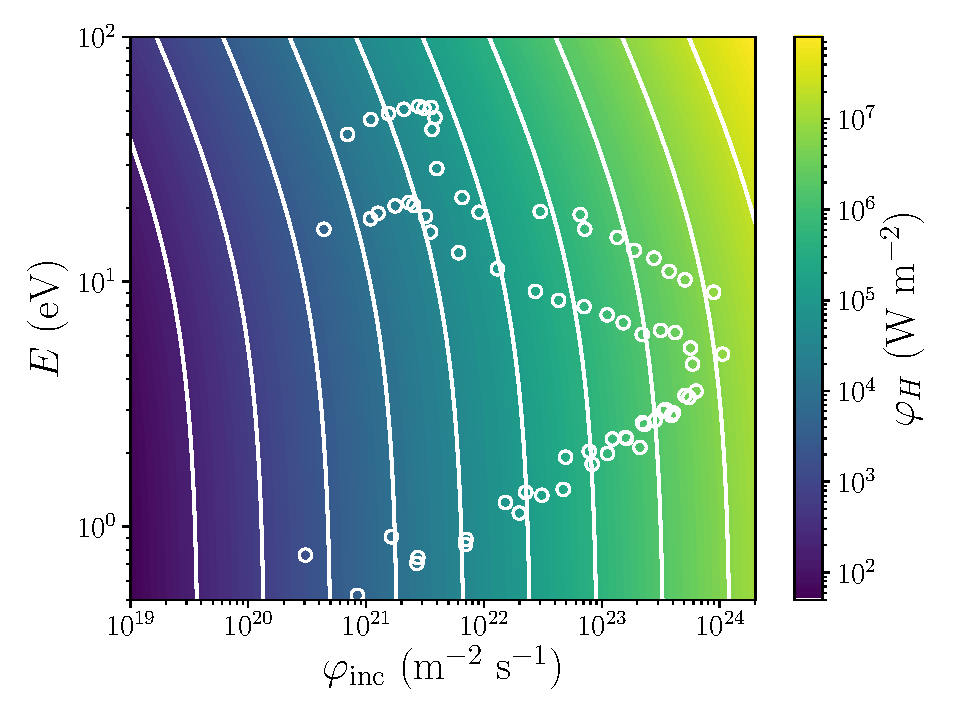
\includegraphics[width=\linewidth]{Figures/Chapter3/monoblocks/parametric_study/phi_H_phi_E.pdf}
%         \caption{Surface heat flux}
%         \label{fig:phi_H phi E}
%     \end{subfigure}%
%     \begin{subfigure}{0.5\linewidth}
%         \centering
%         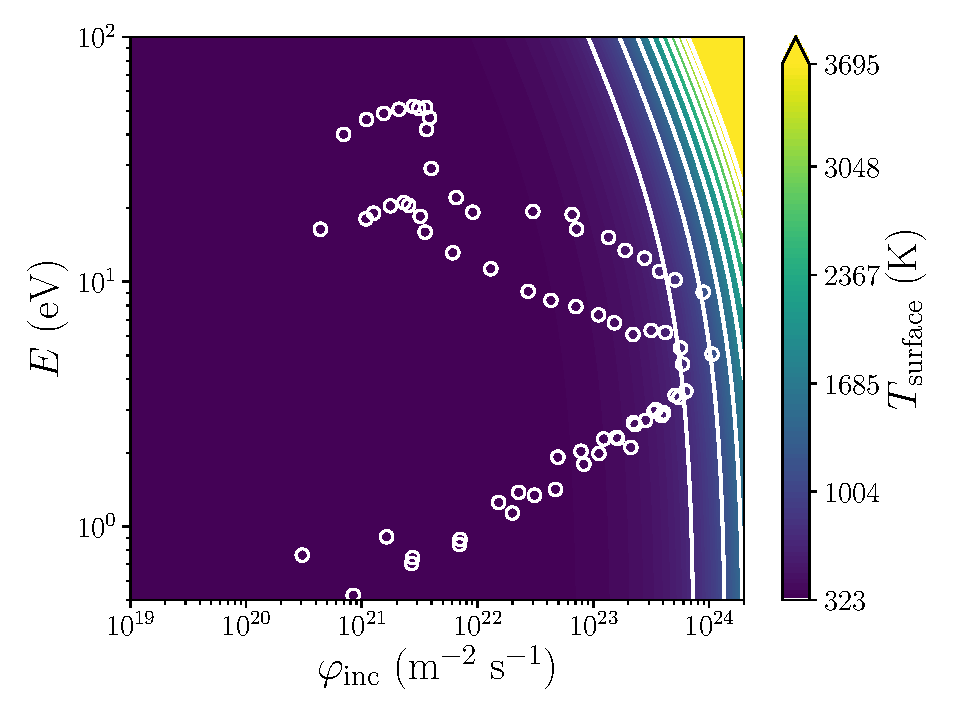
\includegraphics[width=\linewidth]{Figures/Chapter3/monoblocks/parametric_study/T_phi_E.pdf}
%         \caption{Surface temperature}
%         \label{fig:T_surf phi E}
%     \end{subfigure}
%     \begin{subfigure}{0.5\linewidth}
%         \centering
%         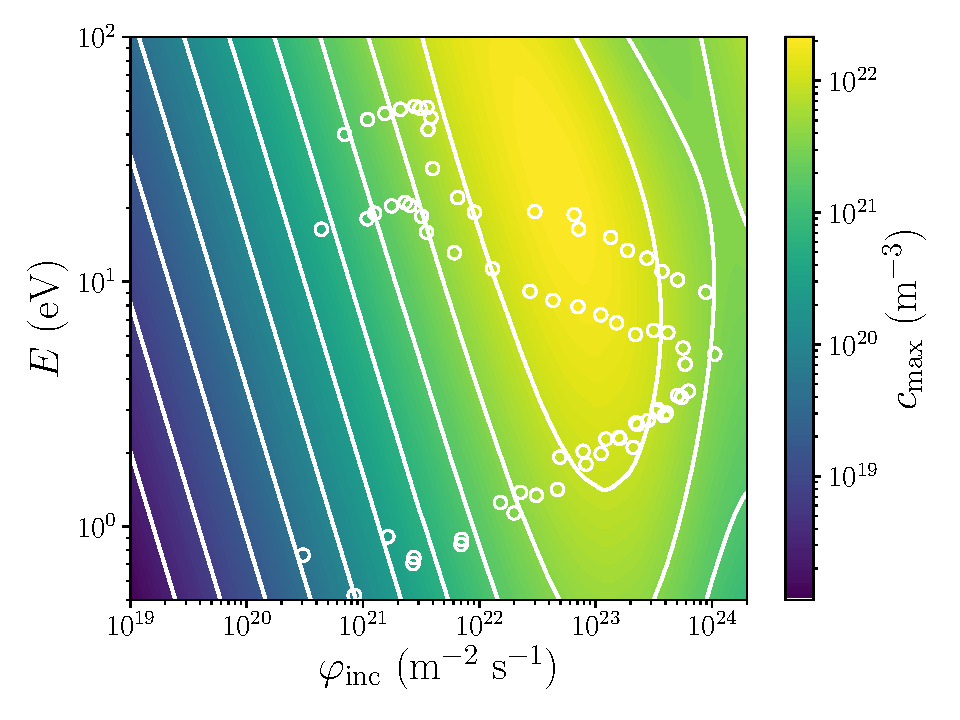
\includegraphics[width=\linewidth]{Figures/Chapter3/monoblocks/parametric_study/c_max_instantaneous.pdf}
%         \caption{Surface concentration}
%         \label{fig:c_max_instantaneous}
%     \end{subfigure}%
%     \begin{subfigure}{0.5\linewidth}
%         \centering
%         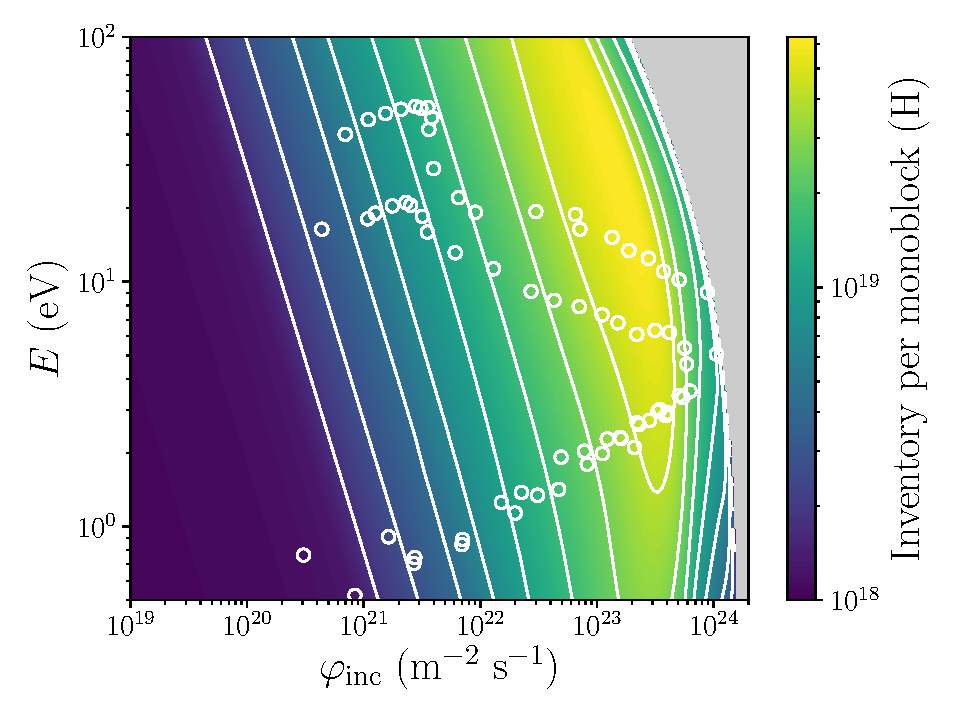
\includegraphics[width=\linewidth]{Figures/Chapter3/monoblocks/parametric_study/inventory_phi_E.pdf}
%         \caption{Monoblock inventory}
%         \label{fig:inventory phi E}
%     \end{subfigure}
%     \caption{$\varphi_H$, $T_\text{surface}$, $c_\mathrm{max}$ and inventory per monoblock as a function of $\varphi_\mathrm{inc}$ and $E$. Inventory has not been calculated for surface temperature above \SI{1200}{K} (greyed region). White circles correspond to points on ITER divertor using the divertor plasma parameters from SOLPS \cite{bonnin_presentation_2016} calculations (see Section \ref{ITER application}).}
%     \label{fig:phi_H T_surf c_max}
% \end{figure*}

% One must be aware that above \SI{1500}{K}, W recrystallisation can occur and H transport will strongly be affected.
% The hypothesis made above as well as material properties may then not be valid.
% Because of the trade-off between the amount of implanted particles and the resulting heat flux, the maximum value of $c_{\mathrm{max}}$ was found to be \SI{2e22}{m^{-3}} around $(\varphi_\mathrm{inc}, E)=(\SI{8e22}{m^{-2}.s^{-1}}, \SI{20}{eV})$.
% Considering the previously calculated response of the monoblock to $c_\mathrm{surface}$ and $T_\mathrm{surface}$ (see Figure \ref{fig:inventory T c}), the inventory as a function of $\varphi_\mathrm{inc}$ and $E$ was computed (see Figure \ref{fig:inventory phi E}).
% The inventory values have not been calculated for surface temperatures above \SI{1200}{K}.
% Again a trade-off was found between implanted particle flux and surface temperature.
% Indeed, the maximum inventory was not found at regions where the incident flux is maximum but rather at regions where $c_\mathrm{surface}$ is maximum and $T_\mathrm{surface}$ is minimum as seen in previous 1D studies \sidecite{hodille_estimation_2017}.

% Each white circle in Figure \ref{fig:phi_H T_surf c_max} corresponds to a point along a poloidal section of the ITER divertor for which implanted particle flux and ion energy were calculated with SOLPS \sidecite{bonnin_presentation_2016} for a partially detached plasma scenario.
% This scenario corresponds to a $Q=10$ discharge with a neutral pressure of \SI{8.6}{Pa} \sidecite{pitts_physics_2019}.


% \begin{figure*} [t]
%     \centering
%     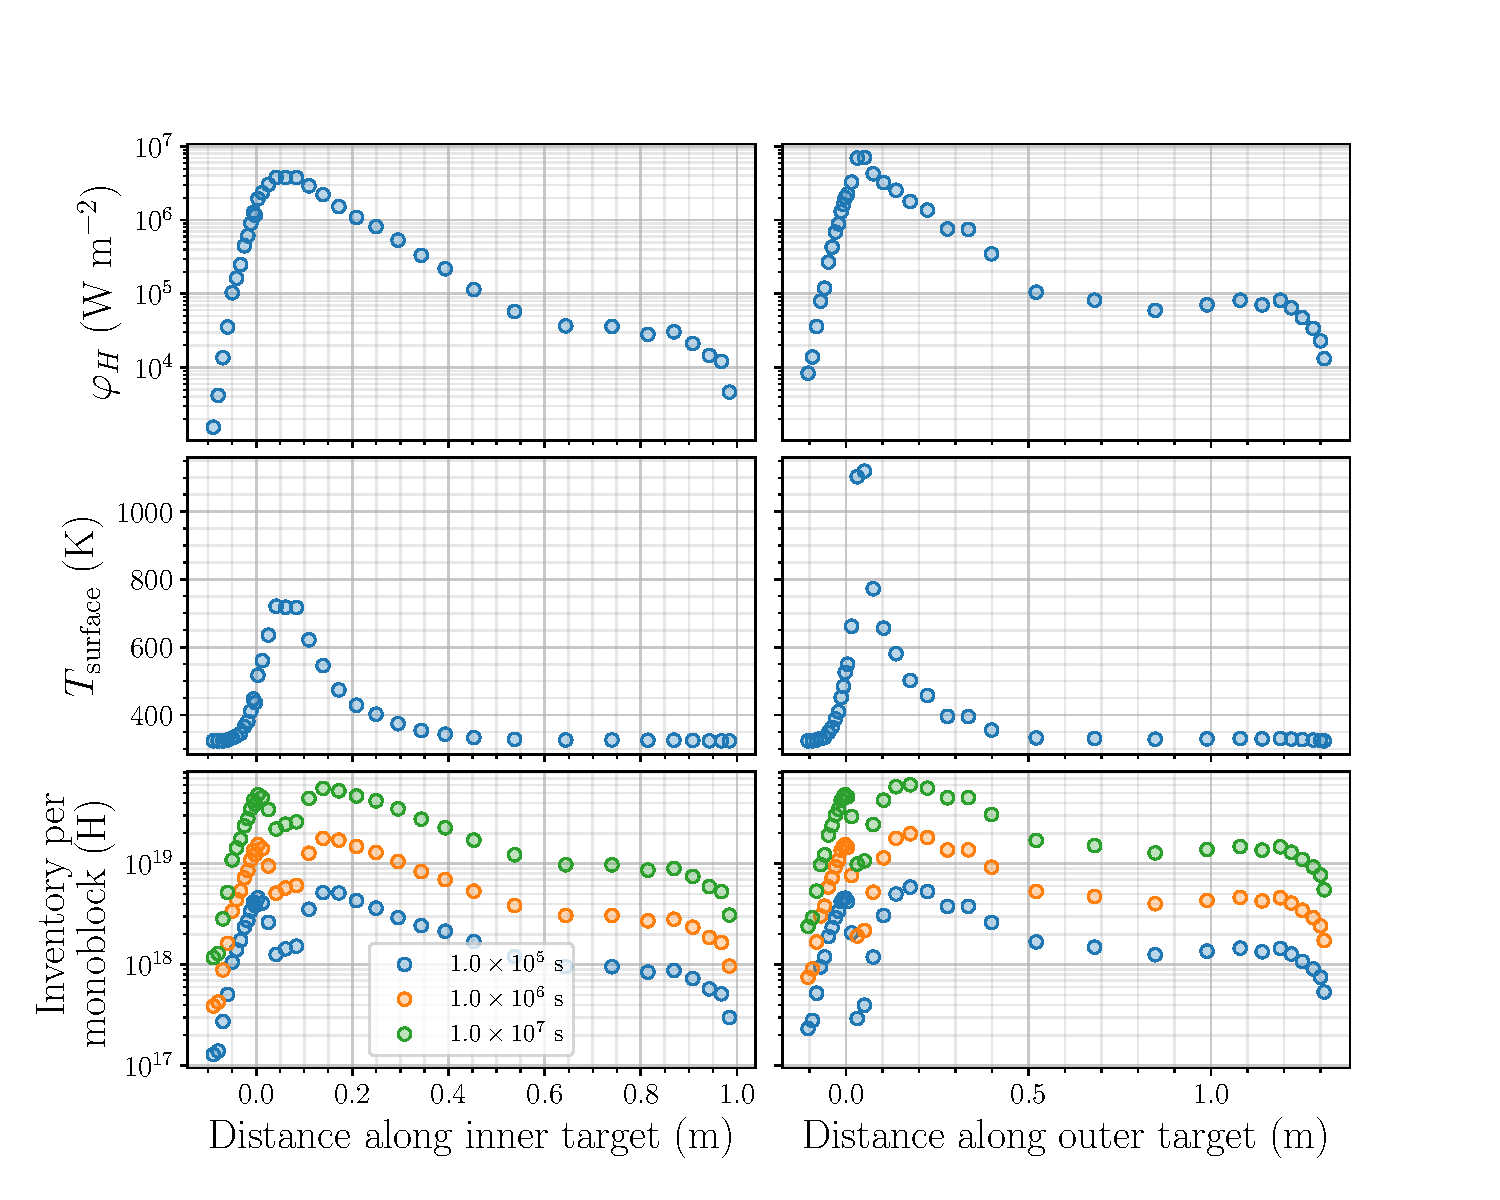
\includegraphics[width=0.8\linewidth]{Figures/Chapter3/monoblocks/parametric_study/along_divertor.pdf}
%     \caption{Evolution of $\varphi_H$ (top), $T_\mathrm{surface}$ (middle) and inventory (bottom) after several exposure times along a poloidal section of the divertor for inner vertical target and outer vertical target.}
%     \label{fig:along divertor}
% \end{figure*}

% As expected the highest surface temperatures and heat loads were located on strike points and most of the zones on the divertor were found to stay at coolant temperature (see Figure \ref{fig:along divertor}).
% The maximum hydrogen content is approximately \SI{6e19}{H} per monoblock after a \SI{e7}{s} exposure.
% As explained in the previous section, the maximum inventory is not necessarily in the region where the flux is maximum as it induces a higher temperature which will tend to increase detrapping: strike points are not where hydrogen is trapped the most.
% Instead, the maximum inventory is reached about \SI{5}{cm} away from the strike points where the temperature and the fluxes are high enough to guarantee a strong source of mobile particle but the temperature is not high enough to trigger detrapping.

% For all points on the divertor, the inventory evolved as $a \cdot t^b$ as shown in Figure \ref{fig:inv_vs_time} for particular points on the inner vertical target ($x=0.03$ m is close to the strike point).
% The coefficient $b$ is maximum on strike points reaching 0.75 (see Figure \ref{fig:a_b_along_div}).
% In other regions, $b$ is closer to 0.5.
% This result can be explained by the non-homogeneous temperature field in monoblocks with high heat loads.
% For monoblocks with a high surface temperature, as hydrogen penetrates deeper into the bulk, the bulk temperature decreases (see Figure \ref{fig:T field 10 MW}) leading to an increase of the trap occupancy \sidecite{hodille_estimation_2017}.
% The exponent $b$ is therefore higher than $0.5$.
% For monoblock where $T_\mathrm{surface} \approx T_\mathrm{coolant}$ on the other hand, the temperature is homogeneous in the whole domain and $b=0.5$.
% This corresponds to a diffusion-limited behaviour.

% The temperature is close to $T_\mathrm{coolant}$ and the trap occupancy is therefore close to one in the whole domain which is not the case for regions near strike points where temperature fields are non-uniform.

% \begin{figure} [t]
%     \centering
%     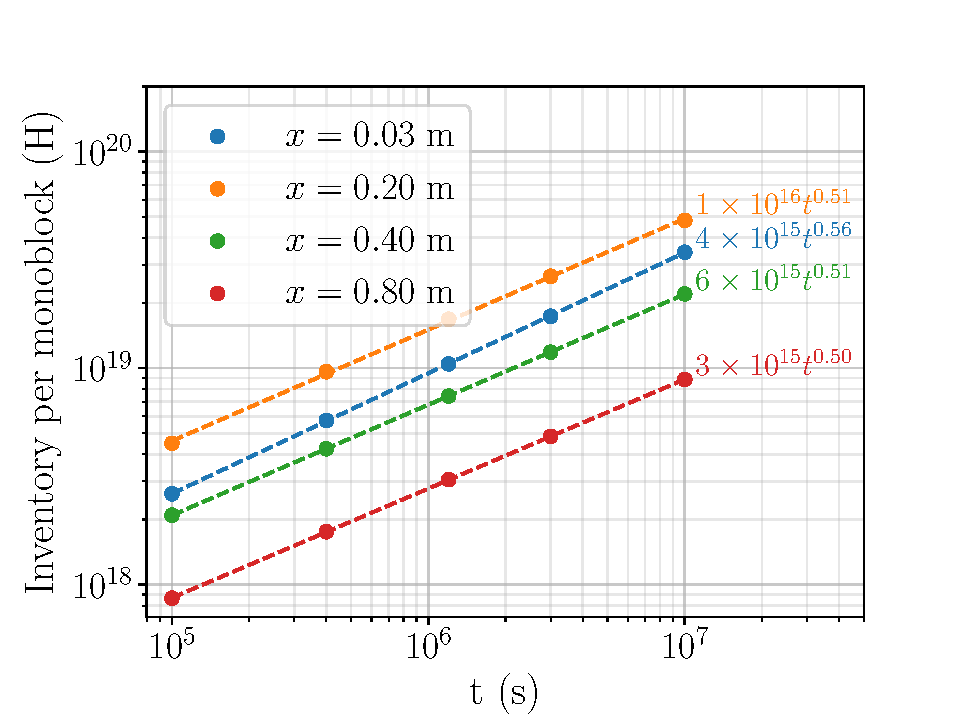
\includegraphics[width=\linewidth]{Figures/Chapter3/monoblocks/parametric_study/inventory_vs_time.pdf}
%     \caption{Temporal evolution of hydrogen inventory in monoblocks at several locations on inner vertical target of ITER divertor}
%     \label{fig:inv_vs_time}
% \end{figure}


% \begin{figure*} [h]
%     \centering
%     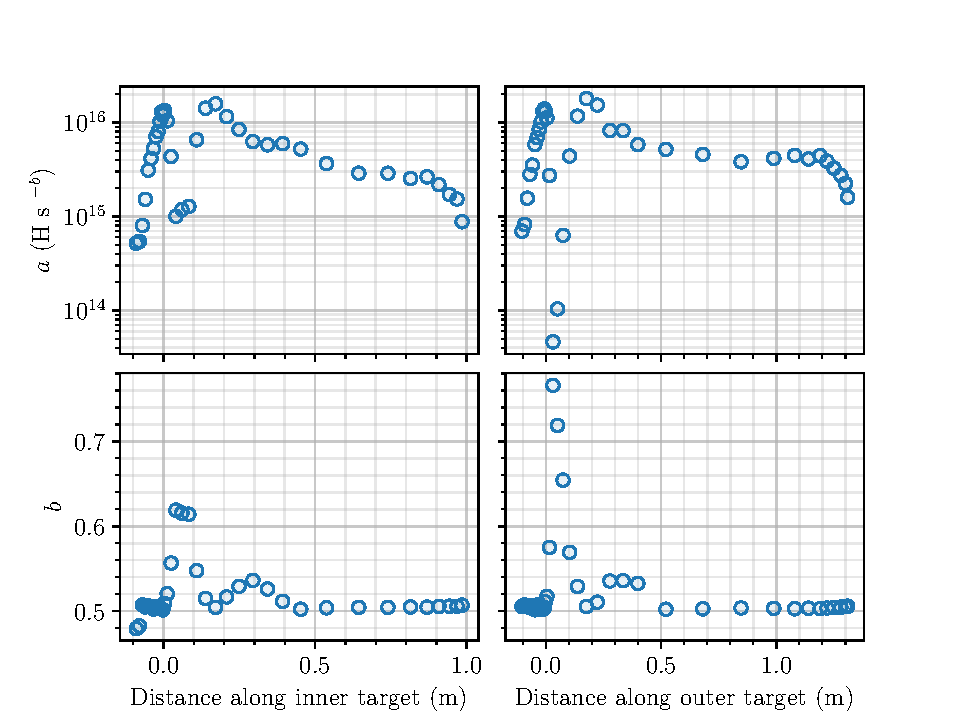
\includegraphics[width=0.8\linewidth]{Figures/Chapter3/monoblocks/parametric_study/a_b_along_div.pdf}
%     \caption{Evolution of coefficients $a$ and $b$ along a poloidal section of the divertor. Inventory evolves as $a\cdot t^b$ (H).}
%     \label{fig:a_b_along_div}
% \end{figure*}

% One can obtain the inventory in the whole divertor by integrating the results obtained in Figure \ref{fig:along divertor} over the tokamak as follow:

% \begin{eqnarray}
%     \mathrm{inv_{divertor}} = N_\mathrm{cassettes}
%     \cdot \left(N_\mathrm{PFU-IVT} \cdot \int \mathrm{inv_{IVT}}(x)\: dx + N_\mathrm{PFU-OVT} \cdot\int \mathrm{inv_{OVT}}(x) \: dx \right)
% \end{eqnarray}
% with $N_\mathrm{cassettes}=54$ the number of cassettes, $N_\mathrm{PFU-IVT}=16$ and $N_\mathrm{PFU-OVT}=22$ the number of plasma facing units per cassette on the inner and outer targets respectively, $\mathrm{inv_{IVT}}$ and $\mathrm{inv_{OVT}}$ the hydrogen inventory profile along the inner and outer targets respectively and $x$ the distance along the targets.

% \begin{figure} [h]
%     \centering
%     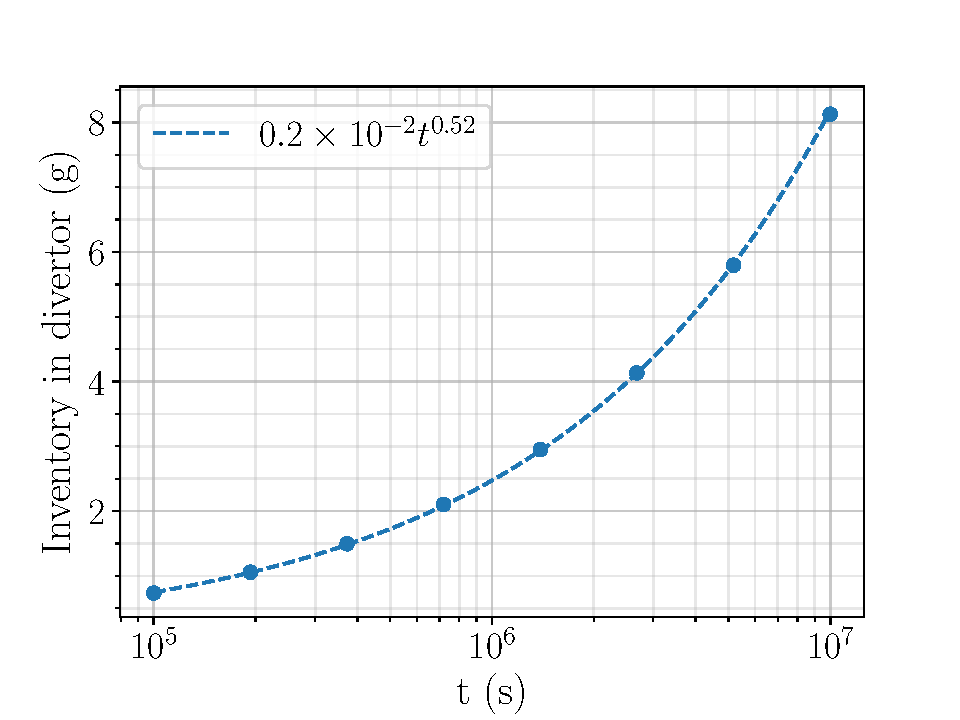
\includegraphics[width=\linewidth]{Figures/Chapter3/monoblocks/parametric_study/inventory_divertor.pdf}
%     \caption{Temporal evolution of hydrogen inventory in the whole divertor}
%     \label{fig:inventory divertor}
% \end{figure}

% After a \SI{e7}{s} exposure, hydrogen inventory is estimated at approximately \SI{8}{g} (see Figure \ref{fig:inventory divertor}) which is relatively low considering the ITER in-vessel limit and the elapsed time.
% De Temmerman \textit{et al} showed that retention in ITER can reach \SI{0.3}{g} per \SI{400}{s} discharge when taking into account Be deposits.

\begin{figure}[h!]
    \centering
    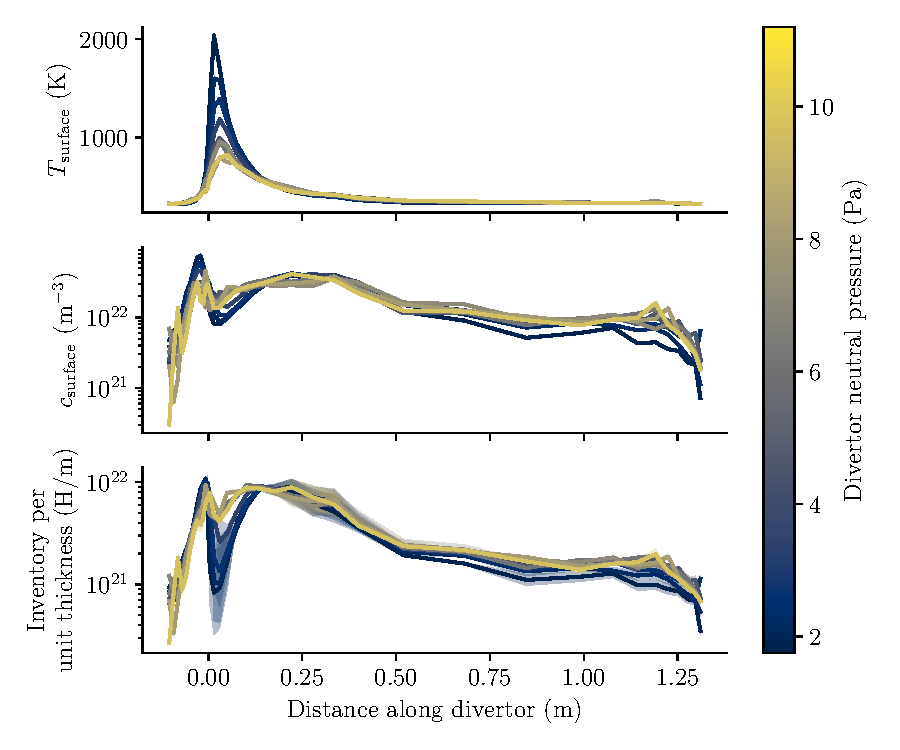
\includegraphics[width=\linewidth]{Figures/divertor/ITER/inventory_along_outer_divertor.pdf}
    \caption{Surface temperature, surface concentration and inventory along ITER outer vertical target with neutral pressures varying from \SI{2}{Pa} to \SI{11}{Pa}. The area corresponds to the 95\% confidence interval.}
    \label{fig: distrib outer target}
\end{figure}


\begin{figure}[h]
    \centering
    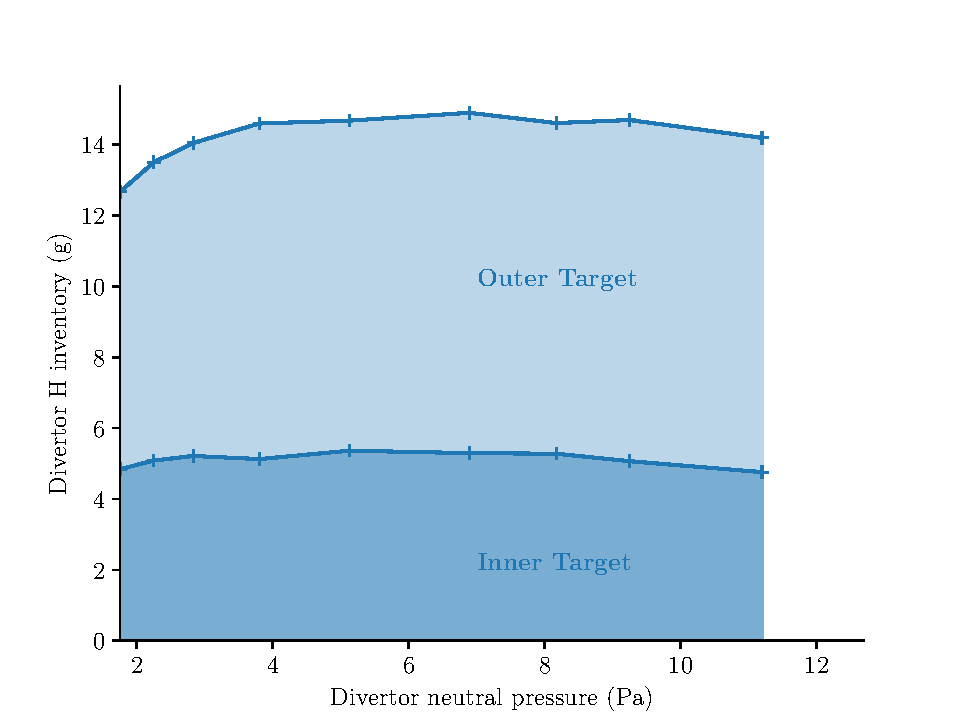
\includegraphics[width=\linewidth]{Figures/divertor/ITER/inventory_vs_divertor_pressure.pdf}
    \caption{Hydrogen inventory in the ITER divertor as a function of neutral pressure after \SI{e7}{s} of exposure (approximately 25 000 discharges).}
    \label{fig: inventory vs neutral pressure}
\end{figure}


\begin{figure}[h!]
    \centering
    \begin{subfigure}{\linewidth}
        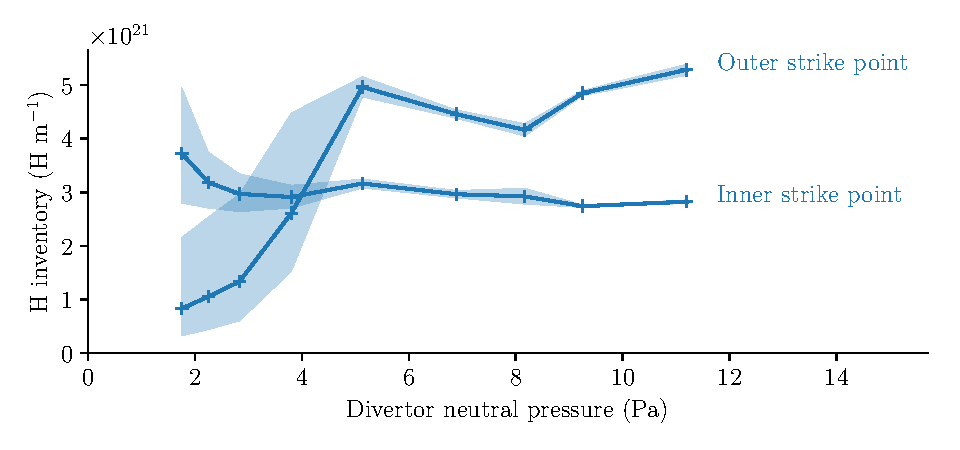
\includegraphics[width=\linewidth]{Figures/divertor/ITER/inventory_at_strike_points.pdf}
        \caption{Inventory per unit thickness after \SI{e7}{s} of exposure (approximately 25 000 discharges). Area corresponds to the 95\% confidence interval.}
        \label{fig: local inventory neutral pressure}
    \end{subfigure}
    \begin{subfigure}{\linewidth}
        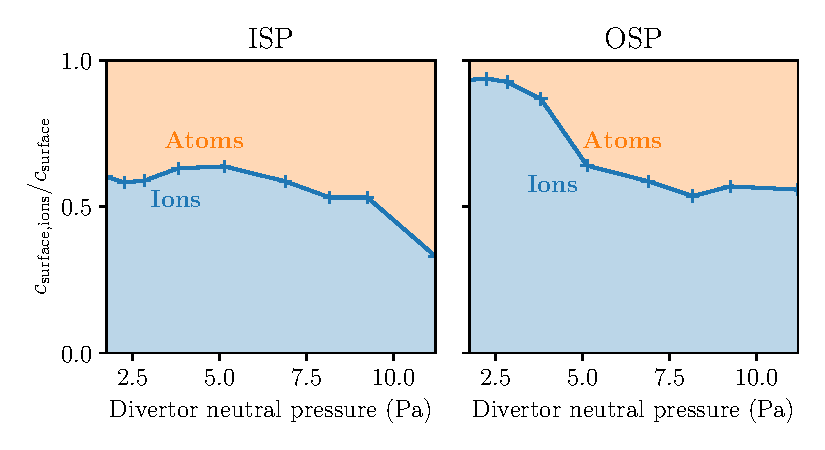
\includegraphics[width=\linewidth]{Figures/divertor/ITER/ratio_ions_atoms.pdf}
        \caption{Contribution of ions to the surface concentration of H.}
        \label{fig: ion contribution neutral pressure}
    \end{subfigure}%
    \caption{H retention at the strike points (defined as maximum temperature) as a function of the divertor neutral pressure.}
\end{figure}

\begin{figure}[h!]
    \centering
    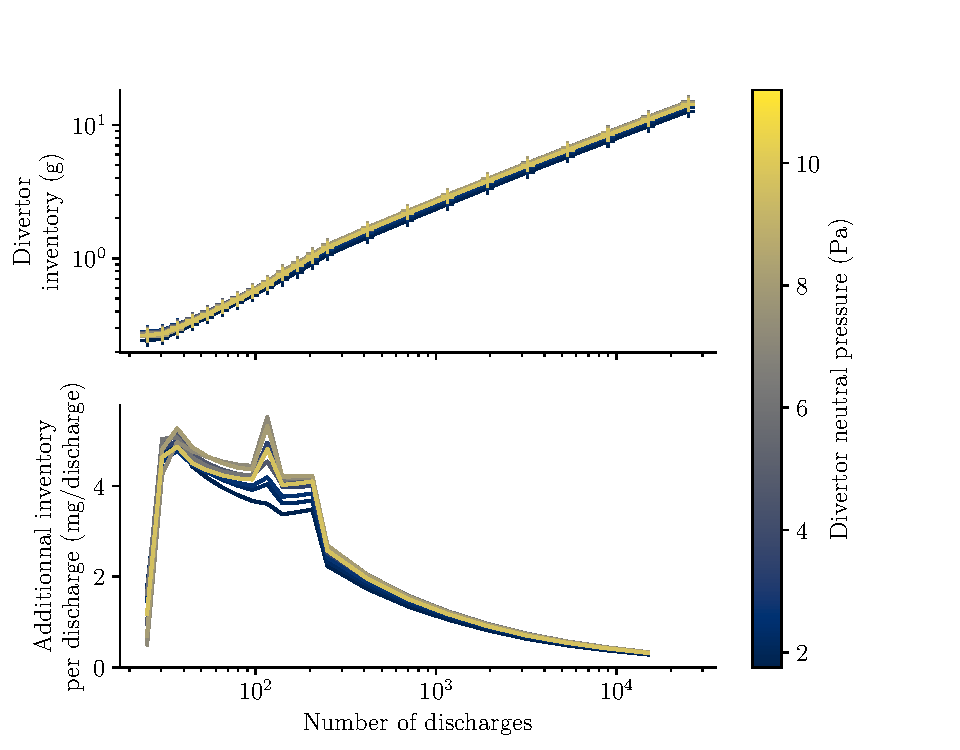
\includegraphics[width=\linewidth]{Figures/divertor/ITER/inventory_vs_time.pdf}
    \caption{Evolution of the H inventory of the ITER divertor with the number of \SI{400}{s} discharges.}
    \label{fig: iter vs time}
\end{figure}


% peak temperature
Peak temperatures at strike points increased when decreasing the divertor neutral pressure (see Figure \ref{fig: distrib outer target}).
The peak temperature at the outer strike point reached \SI{2000}{K} at \SI{2}{Pa} and more than \SI{1000}{K} at the inner strike point, which is in accordance with the results obtained by Pitts \textit{et al} \sidecite{pitts_physics_2019}.

% global inventory
The inventory in the whole divertor is computed as follow:
\begin{equation}
    \mathrm{inv_{divertor}} = N_\mathrm{cassettes} \cdot \left( N_\mathrm{PFU-IVT} \cdot \int \mathrm{inv_{IVT}}(x)\: dx + N_\mathrm{PFU-OVT} \cdot\int \mathrm{inv_{OVT}}(x) \: dx \right)
\end{equation}
with $N_\mathrm{cassettes}=54$ the number of cassettes, $N_\mathrm{PFU-IVT}=16$ and $N_\mathrm{PFU-OVT}=22$ the number of plasma facing units per cassette in the inner and outer targets respectively, $\mathrm{inv_{IVT}}$ and $\mathrm{inv_{OVT}}$ the hydrogen inventory profile along the inner and outer targets respectively and $x$ the distance along the targets.

The inventory in the outer target was found to be nearly twice that of the inner target.
This is largely explained by the larger number of plasma facing units in the outer target and therefore a greater exposed surface.
The global inventory increased with the divertor neutral pressure and a roll-over is observed above \SI{7}{Pa} (see Figure \ref{fig: inventory vs neutral pressure}).
This roll-over is consistent with the results obtained in \sidecite{pitts_physics_2019}.
The inventory increase was found to be more important in the outer vertical target.
This was explained by the fact that the plasma is more detached at the inner target.
Therefore the surface temperature reduction is more significant in the outer vertical target and the surface concentration is increased (see Figure \ref{fig: distrib outer target}).

The maximum inventory was found at around \SI{7}{Pa} and was approximately \SI{14}{g} of H, which is well below the ITER in-vessel safety limit of tritium (\SI{1}{kg}), especially considering only half of this quantity will be tritium.
This is especially true considering that this was for a very long exposure time of \SI{e7}{s}, which corresponds to 25 000 pulses of \SI{400}{s}.


% local inventories
The inventory at the inner and outer strike points globally increases with the divertor neutral pressure (see Figure \ref{fig: local inventory neutral pressure}).
The contribution of ions to the surface concentration at the inner strike point is around 50 \% and tends to decrease with increasing neutral pressure (see Figure \ref{fig: ion contribution neutral pressure}).
At low divertor neutral pressure, the contribution of ions at the outer strike point is around 90 \% and tends to decrease with increasing neutral pressure.
This can be explained by the fact that in both inner and outer targets, the integrated flux of ions decreases with increasing neutral pressure whereas the integrated flux of atoms increases, leading to a greater proportion of neutral particles.

% temporal evolution
For all divertor neutral pressures, the temporal evolution of the divertor inventory is approximately the same (see Figure \ref{fig: iter vs time}).
The additional inventory per \SI{400}{s} discharge was found to decrease with time.
Past 300 discharges, the additional inventory per discharge decreases with the number of discharges.
The maximum is around \SI{5}{mg/discharge} between 30 and 100 discharges.

\section{WEST results}

All the computations have been made for very long exposure times (\SI{e7}{s}) in order to better visualise trends.
Even though cycling can have an effect on H outgassing at the monoblock plasma facing surface, it was shown in \sidecite{hodille_modelling_2021} that the evolution of the monoblock inventory with the fluence was not affected.
Moreover, it can be shown that the divertors inventories evolve with a power law dependence of time.

\subsection{Influence of the input power}

The input power was varied between \SI{0.49}{MW} and \SI{2.0}{MW}.
Two puffing rate values were used: \SI{2.5e21}{molecule.s^{-1}} and \SI{4.4e21}{molecule.s^{-1}}.

\begin{figure}[h]
    \centering
    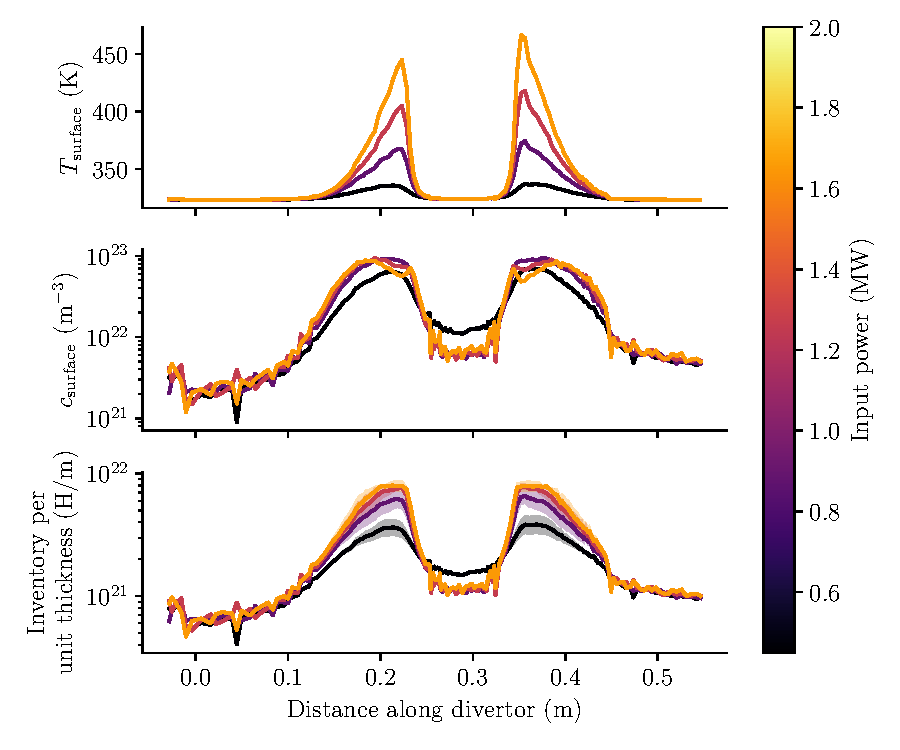
\includegraphics[width=\linewidth]{Figures/divertor/WEST/inventory_along_divertor_input_power.pdf}
    \caption{Distribution of surface temperature $T_\mathrm{surface}$, surface concentration $c_\mathrm{surface}$ and inventory along the WEST divertor with input powers varying from \SI{0.49}{MW} to \SI{2.0}{MW} with a puffing rate of \SI{2.5e21}{molecule.s^{-1}}.}
    \label{fig:divertor distr power scan}
\end{figure}

\begin{figure}[h]
    \centering
    \begin{subfigure}{\linewidth}
        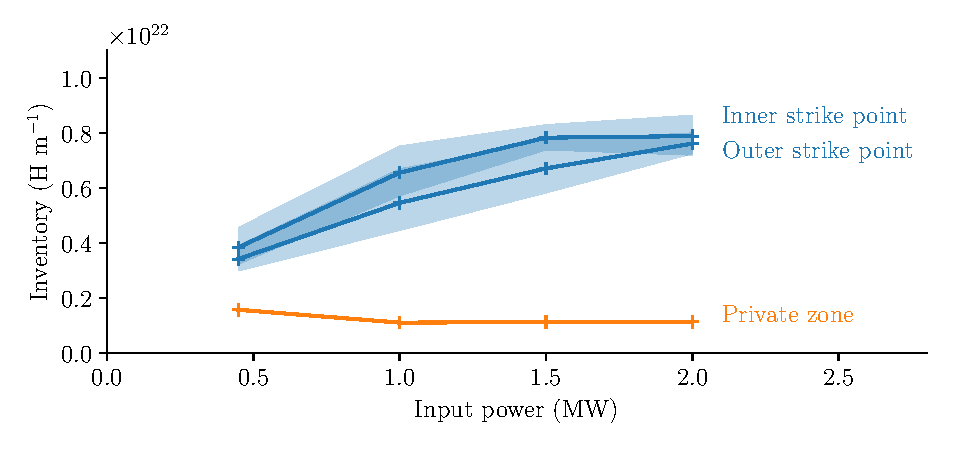
\includegraphics[width=\linewidth]{Figures/divertor/WEST/inventory_at_sps_and_private_zone_vs_input_power.pdf}
        \caption{Inventory per unit thickness after \SI{e7}{s} of exposure. The area corresponds to the 95\% confidence interval.}
        \label{fig: local retention vs input power}
    \end{subfigure}
    \begin{subfigure}{\linewidth}                          
        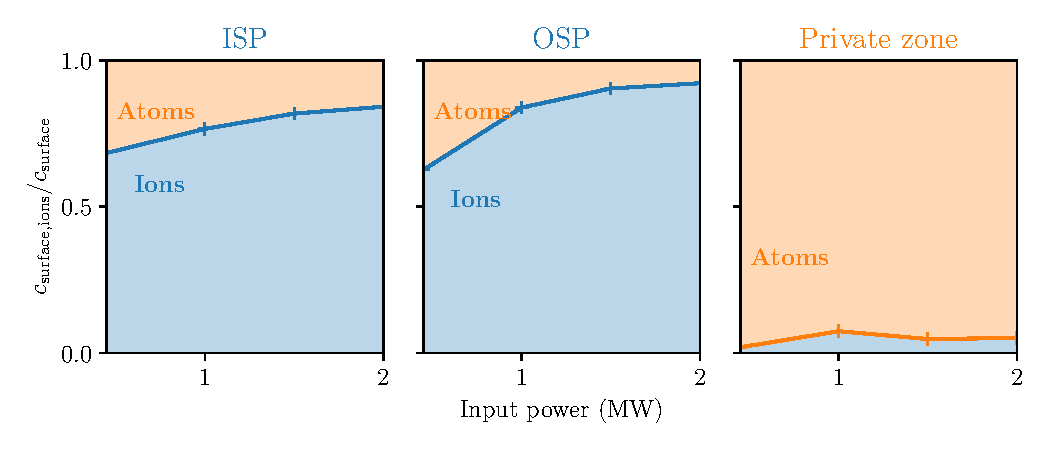
\includegraphics[width=\linewidth]{Figures/divertor/WEST/ions_ratio_vs_input_power.pdf}
        \caption{Contribution of ions to the surface concentration of H. ISP and OSP stand for Inner Strike Point and Outer Strike Point respectively.}
        \label{fig: ion ration vs input power}
    \end{subfigure}%
    \caption{H inventory at the strike points and in the private zone as a function of the input power with a puffing rate of \SI{2.5e21}{molecule.s^{-1}}.}
\end{figure}

\begin{figure}
    \centering
    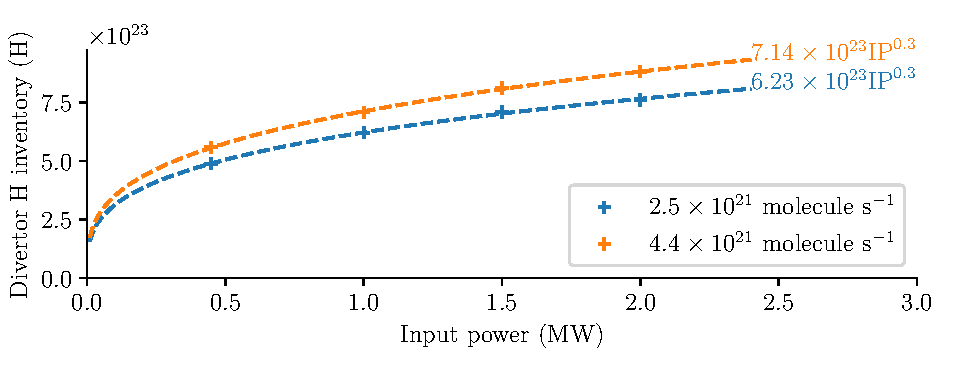
\includegraphics[width=\linewidth]{Figures/divertor/WEST/inventory_vs_input_power.pdf}
    \caption{Evolution of the WEST divertor inventory as a function of input power for several puffing rates.}
    \label{fig:inventory vs input power}
\end{figure}

% \begin{figure*}[h]
%     \centering
%     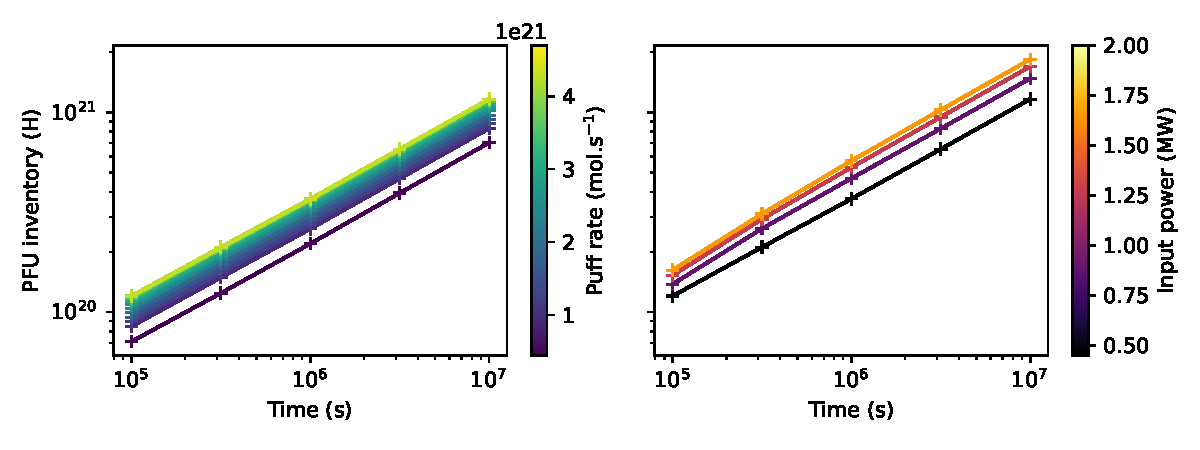
\includegraphics[width=0.8\linewidth]{Figures/divertor/WEST/inventory_vs_time_west.pdf}
%     \caption{Temporal evolution of PFU inventories for different values of puffing rate (left) and input power (right).}
%     \label{fig:temporal evolution west}
% \end{figure*}

% local inventories
The maximum retention was found to be located at the strike points (see Figure \ref{fig:divertor distr power scan}).
The inventory at the outer strike point was higher than at the inner strike point.
The retention at the strike points was found to increase with the input power whereas it slightly decreased in the private zone (see Figure \ref{fig: local retention vs input power}).
This was explained by an attachment of the plasma decreasing the particle flux in the private zone.
Since the surface temperature is constant, this leads to a decrease in the surface concentration of hydrogen as seen on Figure \ref{fig:divertor distr power scan}.
On the other hand, the increasing temperature at the strike points only enhanced the diffusion process while remaining low enough so that hydrogen could get trapped.

The total inventory in the WEST divertor is computed as follows:
\begin{equation}
    \mathrm{inv}_\mathrm{divertor} = N_\mathrm{PFU} \cdot \int \mathrm{inv}_\mathrm{PFU}(x)\: dx
    \label{eq: inventory WEST}
\end{equation}
where $N_\mathrm{PFU} = 480$ is the number of PFU (Plasma Facing Units) in WEST, $\mathrm{inv}_\mathrm{PFU}$ is the inventory per unit thickness in \si{H.m^{-1}} (see Figure \ref{fig:divertor distr power scan}) and $x$ the distance along the target in \si{m}.

The divertor inventory increased with the input power (see Figure \ref{fig:inventory vs input power}) and evolved as the power 0.3 of the input power.
The maximum divertor inventory was \SI{8.8e23}{H} at \SI{2.0}{MW} of input power.
This value of input power is still relatively low.
Increasing the puffing rate lead to an increase in the inventory.
This will be explained more thoroughly in Section \ref{density scan}.

At the strike points, the retention is dominated by the ion flux whereas neutrals are dominant in the private zone (see Figure \ref{fig: ion ration vs input power}).
The contribution of ions at the strike points increased with the input power but remained approximately constant in the private zone.

The divertor inventory was found to increase as a power law of time.


\subsection{Influence of the puffing rate} \label{density scan}

A parametric study on the puffing rate was performed.
The puffing rate was varied between \SI{4.4e20}{molecule.s^{-1}} and \SI{4.7e21}{molecule.s^{-1}}.
The input power was fixed to \SI{0.45}{MW}.

\begin{figure}[h]
    \centering
    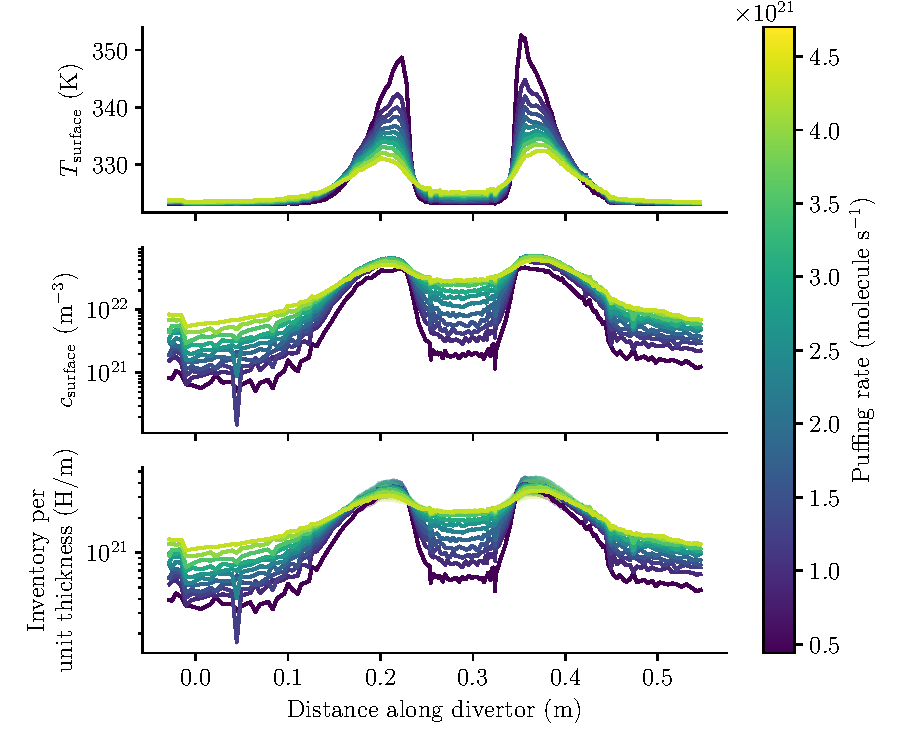
\includegraphics[width=\linewidth]{Figures/divertor/WEST/inventory_along_divertor.pdf}
    \caption{Distribution of surface temperature $T_\mathrm{surface}$, surface concentration $c_\mathrm{surface}$ and inventory along the WEST divertor with a puffing rate varying from \SI{4.4e20}{s^{-1}} to \SI{4.7e21}{s^{-1}} with \SI{0.45}{MW} of input power.}
    \label{fig: divertor distr density scan}
\end{figure}

\begin{figure}[h]
    \centering
    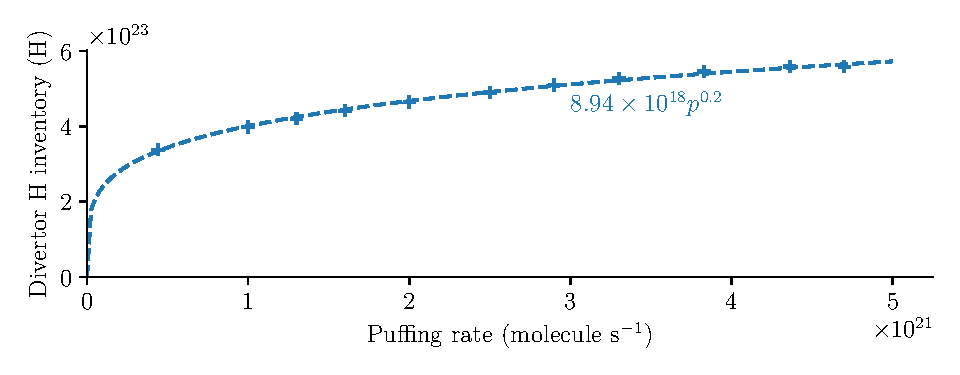
\includegraphics[width=\linewidth]{Figures/divertor/WEST/inventory_vs_puffing_rate.pdf}
    \caption{Evolution of the WEST divertor inventory as a function of puffing rate.}
    \label{fig: inventory vs puffing rate}
\end{figure}

\begin{figure}[h!]
    \centering
    \begin{subfigure}{\linewidth}
        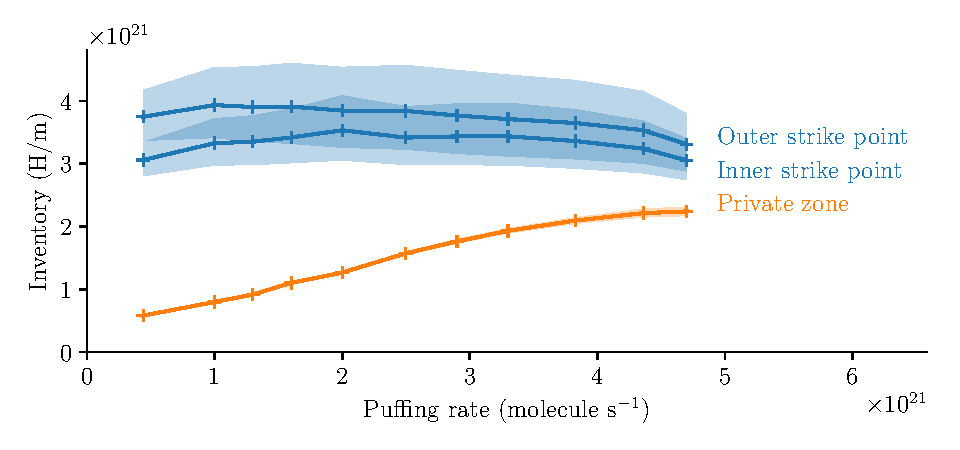
\includegraphics[width=\linewidth]{Figures/divertor/WEST/inventory_at_sp_and_private_zone.pdf}
        \caption{Inventory per unit thickness after \SI{e7}{s} of exposure. The area corresponds to the 95\% confidence interval.}
        \label{fig: local retention vs puffing rate}
    \end{subfigure}
    \begin{subfigure}{\linewidth}
        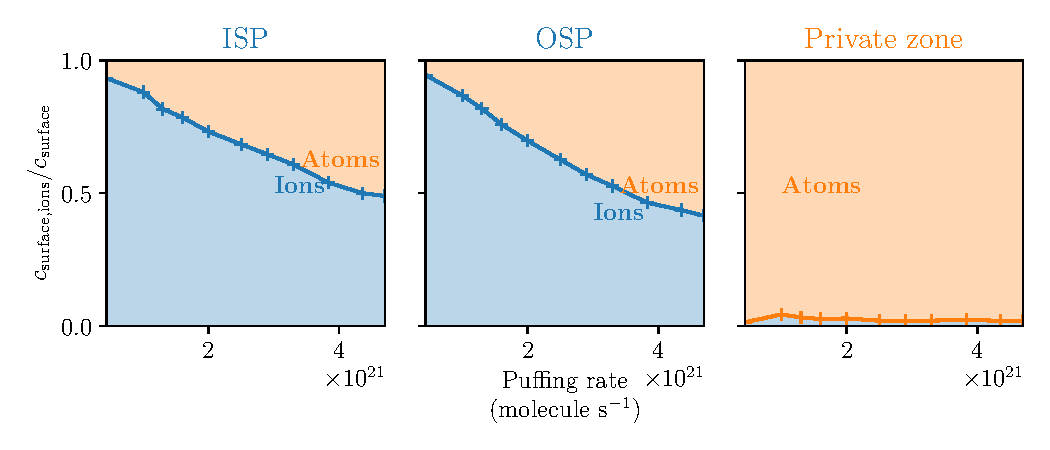
\includegraphics[width=\linewidth]{Figures/divertor/WEST/ion_ratio_at_sp_and_private_zone.pdf}
        \caption{Contribution of ions to the surface concentration of H. ISP and OSP stand for Inner Strike Point and Outer Strike Point respectively.}
        \label{fig: ion contribution vs puffing rate}
    \end{subfigure}%
    \caption{H retention at the strike points and in the private zone as a function of puffing rate with \SI{0.45}{MW} of input power.}
\end{figure}

The maximum retention was again located at the strike points for all puffing rates values (see Figure \ref{fig: divertor distr density scan}).
The inventory at the outer strike point was higher than at the inner strike point.
The inventory in the private zone was found to increase with the puffing rate whereas it was almost constant at the strike points (see Figure \ref{fig: local retention vs puffing rate}).
As for the power scan, the ions contribution to the inventory is rather low in the private zone (see Figure \ref{fig: ion contribution vs puffing rate}).
Moreover, the contribution of ions decreases rapidly at the strike points and represents only half of the surface concentration at \SI{4e21}{molecule.s^{-1}}.

The inventory in the whole WEST divertor is computed from Equation \eqref{eq: inventory WEST}.
As for the power scan, the divertor inventory increased as the power 0.2 of the puffing rate (see Figure \ref{fig: inventory vs puffing rate}).
The maximum inventory was found to be \SI{5e23}{H} at \SI{4.7e21}{molecule.s^{-1}}.

The divertor inventory was found to increase as a power law of time.

\section{Summary}


The monoblock behaviour law proposed in \refch{Chapter3} was used to estimate fuel retention in the divertors of WEST and ITER.
Key control parameters were investigated: the input power, the puffing rate and the divertor neutral pressure.
Their impact on the divertor inventory was studied.

It was shown that the inventory in WEST increases as the power $0.3$ of the input power and as the power $0.2$ of the puffing rate.
The inventory in the ITER divertor was found to first increase with the neutral pressure up to \SI{7}{Pa} then decrease, though the variation was smoother.
The inventory in the outer vertical target of the ITER divertor is twice that of the inner vertical target.
These results were in good agreement with the observations made in \sidecite{pitts_physics_2019}.

However, it should be noted that both machines do not operate in the same regime.
While WEST operates at low input power, ITER operates at high input power with a high recycling divertor.
These differences in the operation regime can explain different trends.

The maximum hydrogen inventory in the ITER divertor was approximately \SI{14}{g} after \SI{e7}{s} of continuous plasma exposure (25 000 ITER discharges), which is well below the safety limit (\SI{1}{kg}).
Moreover, since the behaviour law is based on 2D monoblock simulations, this value is a upper estimate.
2D simulations are indeed conservative in terms of inventory (see \refsec{3D edge effects}).

The underlying monoblock model has also a few limitations, as detailed in \refch{Chapter3}.
First, the set of trapping parameters that was used may not be relevant for every region of the divertor.
These properties can however be experimentally estimated.
The accuracy of the results could therefore be improved by running a new batch of FESTIM monoblock simulations with different trapping parameters like neutron-induced traps.

Then, this model does not take into account retention in Be co-deposited layers.
These are expected to be the main driver for H retention in ITER \sidecite{de_temmerman_data_2021}.
However, this work is still relevant for full-W environments like WEST or DEMO.
